\subsection{Dimensiones del Prototipo}

\par 
Las medidas del prototipo son las siguientes:

\begin{figure}[H]
	\centering
	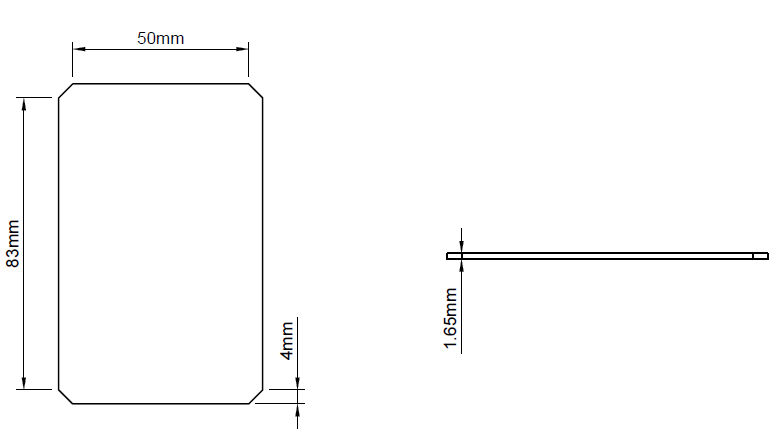
\includegraphics[width=0.8\linewidth]{mediciones1.png}
	\caption{Dibujo y dimensiones de la placa o circuito impreso}
\end{figure}

\par \noindent
Las dimensiones de la placa es lo mas importante a la hora de hacer el armazón. En ella se encuentra el Arduino con sus respectivos módulos y componentes como resistencias, capacitores, interruptor, entrada jack de 3.5 mm y las conexiones con el LCD. La pantalla viene en su propia placa; lo que requiere saber sus dimensiones.

\begin{figure}[H]
	\centering
	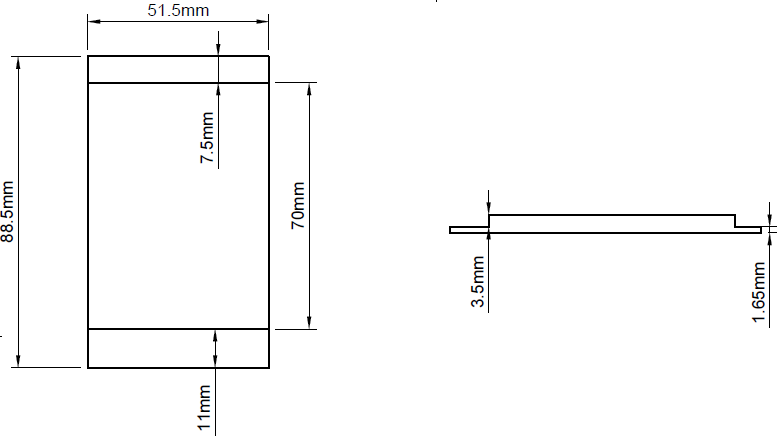
\includegraphics[width=0.8\linewidth]{mediciones2.png}
	\caption{Dibujo y dimensiones de la pantalla LCD y su placa}
\end{figure}

\par \noindent
Siendo la primera iteración de nuestro prototipo se decidió tener una placa para el circuito impreso y otra placa con el LCD. Esto es para que actué como una pieza modular del resto. La conexión de la pantalla con el circuito sera a través de pines. Estos pines le dan una altura al dispositivo. El Armazón por lo tanto debe ser en base a lo siguiente:

\begin{figure}[H]
	\centering
	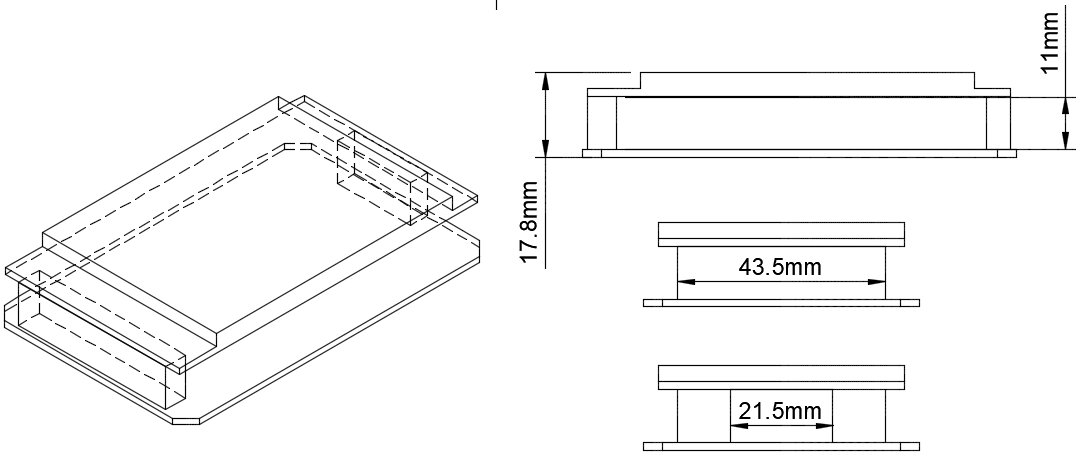
\includegraphics[width=0.8\linewidth]{mediciones3.png}
	\caption{Prototipo ensamblado, base para el diseño del armazón}
\end{figure}

\par \noindent
Ya teniendo encuenta las dimensiones, imagen 4.30. Se procede al bosquejo.

